\documentclass[tikz,border=4pt]{standalone}
% Estilo común de los diagramas de bloques (se usa con \input en cada standalone)
\usepackage[defaultsans,scale=0.92]{lato}
\usepackage{libertinust1math}
\usepackage{xcolor,amsmath}
\usepackage{tikz}
\usetikzlibrary{positioning,arrows.meta,calc,shapes.geometric}
\usepackage{../../notacion}
\definecolor{ctrlazul}{HTML}{1E5AA8}\definecolor{ctrlnoche}{HTML}{14213D}
\definecolor{ctrlcoral}{HTML}{D1495B}\definecolor{ctrlverde}{HTML}{2A9D8F}
\definecolor{ctrlambar}{HTML}{E09F3E}\definecolor{ctrlgris}{HTML}{5C677D}
\definecolor{ctrlvioleta}{HTML}{6C4AB6}\definecolor{ctrlteal}{HTML}{0F7173}
\tikzset{
  >={Stealth[length=2.4mm]}, every node/.style={font=\small},
  bloque/.style={draw=ctrlnoche,fill=ctrlazul!7,thick,rounded corners=1.5pt,minimum height=9mm,minimum width=13mm,inner sep=4pt},
  suma/.style={draw=ctrlnoche,thick,circle,inner sep=0pt,minimum size=6mm},
  senal/.style={->,thick,draw=ctrlnoche},
  rot/.style={font=\footnotesize,text=ctrlgris},
}

\begin{document}
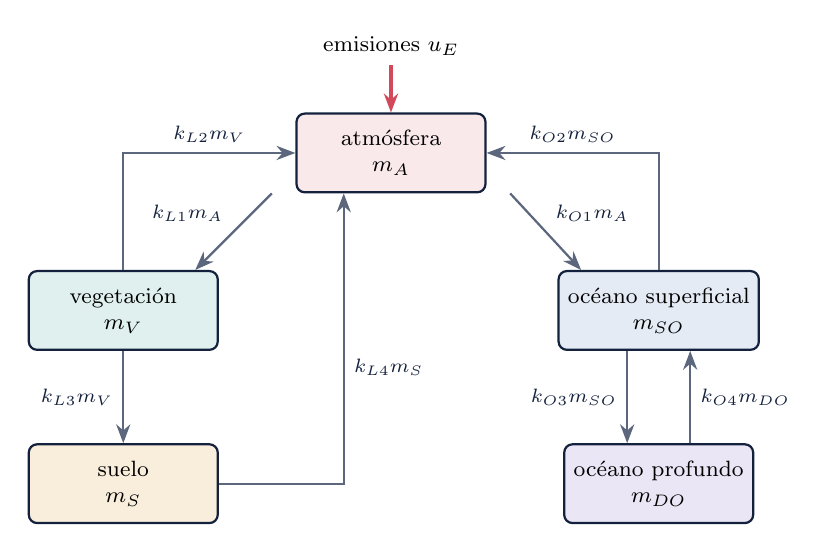
\begin{tikzpicture}[res/.style={draw=ctrlnoche,thick,rounded corners=3pt,minimum width=24mm,minimum height=10mm,align=center,font=\footnotesize},
                    fl/.style={->,thick,draw=ctrlgris},lab/.style={font=\scriptsize,text=ctrlnoche}]
  \node[res,fill=ctrlcoral!12] (A) at (0,0) {atmósfera\\$m_A$};
  \node[res,fill=ctrlverde!15] (V) at (-3.4,-2) {vegetación\\$m_V$};
  \node[res,fill=ctrlambar!18] (S) at (-3.4,-4.2) {suelo\\$m_S$};
  \node[res,fill=ctrlazul!12] (O) at (3.4,-2) {océano superficial\\$m_{SO}$};
  \node[res,fill=ctrlvioleta!14] (D) at (3.4,-4.2) {océano profundo\\$m_{DO}$};
  \node[above=6mm of A,font=\footnotesize] (E) {emisiones $u_E$};
  \draw[->,very thick,ctrlcoral] (E)--(A);
  \draw[fl] ([xshift=-3mm]A.south west)--node[lab,above left]{$k_{L1}m_A$}([xshift=-3mm]V.north east);
  \draw[fl] (V.north)|-node[lab,above,pos=0.75]{$k_{L2}m_V$}(A.west);
  \draw[fl] (V)--node[lab,left]{$k_{L3}m_V$}(S);
  \draw[fl] (S.east)-|node[lab,right,pos=0.7]{$k_{L4}m_S$}([xshift=-6mm]A.south);
  \draw[fl] ([xshift=3mm]A.south east)--node[lab,above right]{$k_{O1}m_A$}([xshift=3mm]O.north west);
  \draw[fl] (O.north)|-node[lab,above,pos=0.75]{$k_{O2}m_{SO}$}(A.east);
  \draw[fl] ([xshift=-4mm]O.south)--node[lab,left]{$k_{O3}m_{SO}$}([xshift=-4mm]D.north);
  \draw[fl] ([xshift=4mm]D.north)--node[lab,right]{$k_{O4}m_{DO}$}([xshift=4mm]O.south);
\end{tikzpicture}
\end{document}
